\documentclass[prb,12pt]{revtex4-2}

%font
% Palatino for main text and math
\usepackage[osf,sc]{mathpazo}

% Helvetica for sans serif
% (scaled to match size of Palatino)
\usepackage[scaled=0.90]{helvet}

% Bera Mono for monospaced
% (scaled to match size of Palatino)
\usepackage[scaled=0.85]{beramono}
%actual packages
\usepackage{amsmath, amssymb,physics,amsfonts,amsthm}
\usepackage{enumitem}
\usepackage[most]{tcolorbox}
\usepackage{cancel}
\usepackage{booktabs}
\usepackage{tikz}
\usepackage{hyperref}
\usepackage{enumitem}
\usepackage{transparent}
\usepackage{float}
\usepackage{multirow}
\newtheorem{Theorem}{Theorem}
\newtheorem{Proposition}{Theorem}
\newtheorem{Lemma}[Theorem]{Lemma}
\newtheorem{Corollary}[Theorem]{Corollary}
\newtheorem{Example}[Theorem]{Example}
\newtheorem{Remark}[Theorem]{Remark}
\theoremstyle{definition}
\newtheorem{Problem}{Problem}
\theoremstyle{definition}
\newtheorem{Definition}[Theorem]{Definition}
\newenvironment{parts}{\begin{enumerate}[label=(\alph*)]}{\end{enumerate}}
%tikz
\usetikzlibrary{patterns}
% definitions of number sets
\newcommand{\N}{\mathbb{N}}
\newcommand{\R}{\mathbb{R}}
\newcommand{\Z}{\mathbb{Z}}
\newcommand{\Q}{\mathbb{Q}}
\newcommand{\C}{\mathbb{C}}
\newcommand*{\circledcirct}{%
	\mathbin{%
		\ooalign{$\circledcirc$\cr\hidewidth$\bullet$\hidewidth}%
	}%
}
\allowdisplaybreaks
\begin{document}
	\title{Lineare Algebra 1 Hausaufgabenblatt Nr. 4}
	\author{Jun Wei Tan}
	\email{jun-wei.tan@stud-mail.uni-wuerzburg.de}
	\affiliation{Julius-Maximilians-Universit\"{a}t W\"{u}rzburg}
	\date{\today}
	\maketitle
%\begin{Problem}
	\begin{parts}
		\item Geben Sie die Definitionen von Gradient, Rotation und Divergenz an.
		\item Wir schreiben die Komponenten des dreidimensionalen Vektorprodukts als
			\[
				(\vec{a}\times \vec{b})_i=\sum_{j,k=1}^3 \epsilon_{ijk}a_jb_k,\] 
				wobei $\epsilon_{ijk}$ der total antisymmetrische Tensor f\"{u}r $\R^3$ ist, mit $\epsilon_{ijk}=1$. Zeigen Sie, dass gilt:
				\begin{align*}
					\sum_{i=1}^3 \epsilon_{ijk}\epsilon_{ilm}=&\delta_{jl}\delta_{km}-\delta_{jm}\delta_{kl}\\
					\frac{1}{2}\sum_{i,j=1}^3 \epsilon_{ijk}\epsilon_{jl}\delta_{kl},
				\end{align*}
				mit $\delta$ dem Kronecker-$\delta$.
			\item Zeigen Sie mit den Formeln aus (b) die folgenden Identitäten für beliebige Vektorfelder $\vec{a},~\vec{b},~\vec{c},~\vec{d}$:
				\begin{align*}
					\vec{a}\cdot(\vec{b}\times\vec{c})&=\vec{b}\cdot (\vec{c}\times \vec{a})=\vec{c}\cdot (\vec{a}\times \vec{b})\\
					\vec{a}\times(\vec{b}\times\vec{c})=&(\vec{a}\cdot\vec{c})\vec{b}-(\vec{a}\cdot\vec{b})\vec{c},\\
					(\vec{a}\times\vec{b})\cdot(\vec{c}\times\vec{d})=*(\vec{a}\cdot\vec{c})(\vec{b}\cdot\vec{d})-(\vec{a}\cdot\vec{d})(\vec{b}\cdot\vec{c})
				\end{align*}
			\item Zeigen Sie damit, dass f\"{u}r beliebige skalare Funktionen $F(\vec{x})$ und Vektorfelder $\vec{A}(\vec{x})$ gilt:
				\begin{align*}
					\curl{\grad{F}}=&0\\
					\div{(\curl{A})}=&0\\
					\curl{\curl{A}}=&\grad{(\div{A})}-\laplacian{A}\\
					\div{(F\vec{A})}=(\grad{F})\cdot\vec{A}+F\div{\vec{A}},
				\end{align*}
				mit $\Delta$ dem Laplace-Operator.
	\end{parts}
\end{Problem} 
\begin{proof}
	\begin{parts}
	\item 
		\begin{align*}
			\text{grad }F=\sum_{i=1}^3 \pdv{F}{x_i}\hat{x}_i\\
			\text{div }\vec{F}=\sum_{i=1}^3 \pdv{F_i}{x_i}\\
			\text{curl }\vec{F}=&\ldots
		\end{align*}
	\item Offensichtlich muss $j\neq k$ und $l\neq m$ sein, ansonsten wäre 1
	\end{parts}
\end{proof}
\begin{Problem}
	
\end{Problem}

%\begin{Problem}
	Betrachten Sie die folgenden Familien von Kraftfeldern auf geeigneten Definitionsbereichen $D_\eta^{(n)}  \subseteq \R^3$
	\begin{align*}
		F_\eta^{(1)}:& D_\eta^{(1)}\ni \va x\to r^\eta\cdot \va x\in \R^3\\
		F_\eta^{(2)}:& D_\eta^{(2)}\ni\va x \to r_{12}^\eta\cdot(x_1\va e_1-x_2\va e_2)\in \R^3\\
		F_\eta^{(3)}:& D_\eta^{(3)}\ni \va x\to r_{12}^\eta\cdot\left( x_2\va e_1-x_1\va e_2 \right) \in\R^3\\
		F_\eta^{(4)}:&D_\eta^{(3)}\ni \va x\to r_{12}^\eta\cdot\left( x_2\va e_1+x_1\va e_2 \right) \in \R^3
	\end{align*}
	wobei $r_{12}=\sqrt{x_1^2+x_2^2} $ und $r=\sqrt{x_1^2+x_2^2+x_3^3} $
	Skizzieren Sie die Felder $\va F_\eta^{(n)}$ als Vektorpfeile in der von den Einheitsvektoren $\va e_1$ und $\va e_2$ aufgespannten Ebene (hier genügt es, zwischen den Fällen $\eta > -1, \eta = -1$ und $\eta < -1$ zu unterscheiden). 
	
	Bestimmen Sie, abhängig von der Potenz $\eta \in \R$,
	\begin{enumerate}
		\item den maximalen Definitionsbereich $D_\eta^{(n)}$,
		\item die maximale Bereiche $C_\eta^{(n)}\subseteq D_\eta^{(n)}$, auf denen $F_\eta^{(n)}$ konservativ ist,
		\item eine Potentialfunktion $V_\eta^{(n)}:C_{\eta}^{(n)}\to \R$ mit $F_\eta^{(n)}=-\grad{V_\eta^{(n)}}$, sofern sie existiert,
		\item das Kurvenintegral
		\[I_\eta^{(n)}(R)=\int_{\gamma_R}\dd{\va\xi}\cdot\va F_\eta^{(n)}(\va\xi)\]
		über den gegen den Uhrzeigersinn umlaufenen Kreis $\gamma_R$ mit Radius $R$ und Mittelpunkt $\va0$ in der von $\va e_1$ und $\va e_2$ aufgespannten Ebene
		\begin{center}
			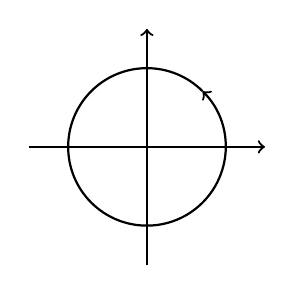
\begin{tikzpicture}
				\draw[thick, ->] (-1.5,0) -- (1.5,0);
				\draw[thick, ->] (0,-1.5) -- (0,1.5);
				\draw[thick, ->] ({1/sqrt(2)},{1/sqrt(2)}) arc (45:405:1);
			\end{tikzpicture}
		\end{center}
	\end{enumerate}
\end{Problem}

%\begin{Problem}
	Let $V$ be a $\mathbb{K}$-valued vector space. A seminorm on $V$ is a homogeneous map $p:V\to [0,\infty)$ satisfying the triangle inequality, i.e.
	\[
	p(v+w)\le p(v)+p(w)
\]
and
\[
p(\lambda v)=|\lambda|p(v)
\]
for any two vectors $v,w\in V$ and every scalar $\lambda\in\mathbb{K}$.
\begin{parts}
	\item Show that the kernel of a seminorm $p$ is a subspace of $V$.

		Given a seminorm $p$, we say that two vectors $v,w\in V$ are equivalent if there is a vector $u\in \text{ker }p$ such that $w=v+u$. Make yourself clear that this yields an equivalence relation on $V$.
	\item Show that the quotient space $V / \text{ker }p:=V / \sim$ carries a canonical linear structure.
	\item Show that the map
		\[
			\overline{p}:V / \text{ker }p\ni [v]\mapsto p(v)
		\]
		yields a well-defined norm on the quotient space.
\end{parts}
\end{Problem}
\begin{proof}
	\begin{parts}
	\item Clear by definition
	\item Also clear
	\end{parts}
\end{proof}
\begin{Problem}\label{pr:funcanalblatt3-2}
	Let $M$ be a topological space. Show that the space $(\mathcal{C}_b(M), \|\cdot\|_\infty)$ of continuous and bounded $\mathbb{K}$-valued functions endowed with the supremum norm is complete.
\end{Problem}

\begin{Problem}
	In this exercise we weaken the conditions of Homework~\ref{pr:funcanalblatt3-2} by considering functions that are only essentially bounded. The goal is to find a suitable seminorm on this function space such that the corresponding quotient becomes a Banach space. But first, we shall settle the term ``essentially bounded''. To this end, we need the following definitions:

	Let $X$ be a set and $\mathfrak{a}\in 2^X$. We call $\mathfrak{a}$ a $\sigma$-algebra if
	\begin{itemize}
		\item $\varnothing\in\mathfrak{n}$,
		\item $X \setminus A\in \mathfrak{a}$ for every $A\in \mathfrak{a}$ and
		\item $\bigcup_{n\in \N} A_n\in \mathfrak{a}$ for every sequence $(A_n)_{n\in \N}\subset \mathfrak{a}$
	\end{itemize}
	The pair $(X, \mathfrak{a})$ is called a measurable space. One can check that for every $A\in \mathfrak{a}$ one obtains a new $\sigma$-algebra $a|_{X\setminus A}\subseteq 2^{X \setminus A}$, where $B\in \mathfrak{a}_{X \setminus A}$iff there is some $C\in \mathfrak{a}$ such that $B=C \setminus A$.

	A function $f: (X, \mathfrak{a})\to \mathbb{K}$ if $f^{-1}(B_r(z))\subseteq \mathfrak{a}$ for every $z\in \mathbb{K}$ and $r>0$. We denote the set of measurable $\mathbb{K}$-valued functions by $\mathcal{M}(X, a)$. Clearly, the restriction of a measurable function $f\in \mathcal{M}(X, a)$ to $X \setminus A$ yields a measurable function $f|_{X \setminus A}\in \mathcal{M}(X \setminus A, \mathfrak{a}|_{X \setminus A})$.

	Finally, a subset $\mathfrak{n}\subseteq \mathfrak{a}$ is called a $\sigma$-ideal if
	\begin{itemize}
		\item $\varnothing \in \mathfrak{n}$,
		\item $\bigcup_{n\in \N} A_n\in \mathfrak{a}$ for every sequence $(A_n)_{n\in \N}\subset \mathfrak{n}$ and
		\item for all $A\in \mathfrak{n}$ and $B\in\mathfrak{a}$ one has the implication $B\subseteq A\implies B \in \mathfrak{n}$.
	\end{itemize}
	\begin{parts}
	\item For $f\in \mathcal{M}(X, \mathfrak{a})$ we define the essential range
		\[
			\text{ess range}(f):=\{z\in \mathbb{K}:f^{-1}(B_r(z))\not\in \mathfrak{n}\text{ for all }r>0\} 
		\]
		and the essential supremum
		\[
			\text{ess sup}(f):=\sup \{|z|:z\in \text{ess range}(f)\} 
		.\] 
		Show that $\text{ess range}(f)\subseteq \mathbb{K}$ is closed and $f^{-1}(\mathbb{K}\setminus\text{ess range}(f))\in \mathfrak{n}$.
	\item Show that two functions $f,g\in \mathcal{M}(X, \mathfrak{a})$ have the same essential range if the essential range of $f-g$ contains only $0$.
	\item The set of essentially bounded functions on $X$ is defined as
		\[
			\mathcal{L}^\infty (X, \mathfrak{a}, \mathfrak{n}):=\{f\in \mathcal{M}(X, a):\|f\|_\text{ess sup}:=\text{ess sup}(f)<\infty\} 
		.\] 
		Show that $\|\cdot\|_\text{ess sup}$ defines a seminorm on $\mathcal{L}^\infty(X, \mathfrak{a}, \mathfrak{n})$ and compute its kernel. Moreover, show that the essential supremum of $f\in \mathcal{L}^\infty(X, \mathfrak{a}, \mathfrak{n})$ is given by
		\[
			\text{ess sup}(f)=C_f:=\inf \{C>0:|f|^{-1}([C,\infty))\in \mathfrak{n}\}  
		.\] 
		Hint: You can use that $\mathcal{M}(X, \mathfrak{a})$ and $\mathcal{L}^\infty(X, \mathfrak{a}, \mathfrak{n})$ are $\mathbb{K}$-vector spaces without proof.
	\item Show that $L^\infty(X, \mathfrak{a}, \mathfrak{n}):= \mathcal{L}^\infty (X, \mathfrak{a}, \mathfrak{n}) / \text{ker}\|\cdot\|_{ess sup}$ is a Banach space, i.e. a complete normed space.

		Hint: Consider the sequence $(f_n)_n$ on a suitable subset of $X$ and copy your proof of Homework~\ref{pr:funcanalblatt3-2}. You can use that a pointwise limit of a sequence of measurable functions is again measurable without proof.
	\end{parts}
\end{Problem}

	The following exercises are intended to understand the London–Pippard phenomenological theory. 
We are going to derive them with a simple model. For that we start considering the supercurrent 
can be thought as a nonviscous charged fluid with field velocity $\vec v(\vec x,t)$, that obeys
\[
\vec j(\vec x,t) = - n_s e \vec v(\vec x,t),
\]
where $n_s$ is the density of the super-electron number density and $-e$ is the electronic charge. 
The continuity equation together with Newton's second law give
\[
\nabla \cdot \vec j = \nabla \cdot \vec v = 0,
\]
\[
\frac{d \vec v}{dt} = -\frac{e}{m}\left( \vec E + \frac{1}{c}\vec v \times \vec h \right),
\]
with $\vec h$ the microscopic field which is larger compared to the atomic size but smaller compared 
to the penetration depth. Notice that this also involves the total derivative with respect to time of 
the velocity and not just its partial (explicit) dependence.

% --------------------------- PROBLEM 1 ---------------------------
\begin{Problem}
	\begin{itemize}
		\item Define the effective field
		\[
		\vec Q = \nabla \times \vec v - \frac{e}{mc}\vec h.
		\]
		
		Together with Maxwell’s equations, derive the dynamical equation for $\vec v$ for a 
		superconducting bulk under the constraint $\vec Q = 0$.  
		\textbf{Hint:} Notice that in Newton's second law equation it was written $d/dt$ and 
		not $\partial/\partial t$. Recall for a field vector which is the relation between those 
		two and use it to get the equation $\partial \vec v/\partial t$.
		
		\item How can we interpret $\vec Q$?
	\end{itemize}
\end{Problem}
\begin{proof}
	First, a comment on the units: Due to the factor of $1 / c$ in the Lorentz force, the equation is written in Gaussian units. We also note that $\vec{h}$ is the ``$B$-field'', i.e. it does not have a prefactor related to the permeability already absorbed in. In these units, the Maxwell's equations are given by
	\begin{align*}
		\div{\vec{E}}&=4\pi\rho \\
		\div{\vec{B}}&= 0 \\
		\curl{\vec{E}}+\frac{1}{c}\pdv{\vec{B}}{t}&= 0 \\
		\curl{\vec{B}} -\frac{1}{c}\pdv{\vec{E}}{t}&=\frac{4\pi}{c}\vec{j}
	\end{align*}
	The material derivative is given by
	\[
		\dv{f}{t} = \pdv{f}{t} + \vec{v}\cdot\grad{f}
	.\] 
	We apply this to $f=\vec{v}$ to get
	\begin{align*}
		\pdv{\vec{v}}{t} + \vec{v}\cdot\grad{\vec{v}}&=-\frac{e}{m}\left( \vec{E} + \frac{1}{c}\vec{v}\times \vec{h} \right) \\
							     &= -\frac{e}{m}\vec{E} - \vec{v}\times(\curl{\vec{v}}) 
	\end{align*}
	We recall a certain lemma, which can be found on lists of vector calculus identities
	\begin{Lemma}
		\[
			\vec{v}\cdot\grad{\vec{v}} = \grad{\left( \frac{v^2}{2} \right)} -\vec{v}\times(\curl{\vec{v}}) 
		.\] 
	\end{Lemma}
	This leads to
	\[
		\pdv{\vec{v}}{t} = \grad{\left( \frac{v^2}{2} \right) }-\frac{e}{m}\vec{E}
	.\] 
	The vector $\vec{Q}$ can be interpreted as a generalised vorticity
	\begin{align*}
		\vec{Q} &= \curl{\vec{v}} - \frac{e}{mc}\vec{h} \\
			&= \curl{\vec{v}} - \frac{e}{mc}\curl{\vec{A}} \\
			&= \curl{\left( \vec{v} - \frac{e}{mc}\vec{A} \right)}.\qedhere  
	\end{align*}
\end{proof}
% --------------------------- PROBLEM 2 ---------------------------
\begin{Problem}
	Now consider a semi-infinite slab in the 3D space that occupies $z > 0$. One of the equations 
	of the previous item can be rewritten as
	\[
	\vec h = -\frac{mc}{n_s e^2}\nabla \times \vec j.
	\]
	
	\begin{itemize}
		\item Rewrite the previous equation using the Maxwell equations for static fields to write $\vec h$ 
		in terms of spatial derivatives of $\vec h$.
		
		\item Consider an applied field $\vec H = H_0 \hat x$ parallel to the surface. Recalling that inside 
		the superconductor the field has to be zero, find an acceptable solution for the microscopic field. 
		What is the penetration depth? Identify the London penetration depth $\lambda_L$.
		
		\item If the slab has a $2d$ thickness, under the same external field, can you find an appropriate 
		solution for $\vec h(z)$? Check that it is a solution of the differential equation that you found before. 
		Consider the mean magnetic field in the superconductor as the spatial average of $h(z)$. 
		What can you say about the Meissner effect when $d \ll \lambda_L$ and $d \gg \lambda_L$?
	\end{itemize}
\end{Problem}
\begin{proof}
	\begin{itemize}
		\item We have the Maxwell's equation
	\[
		\curl{h} = \frac{4\pi}{c} \vec{j}
	.\] 
Then, substituting this in, we get
\begin{align*}
	\vec{h} &= -\frac{mc}{n_s e^2}\curl{\left(\frac{c}{4\pi}\curl{\vec{h}}\right)} \\
		&= -\frac{mc^2}{4\o\pi n_s e^2}(\grad{(\div{\vec{h}})}-\laplacian{\vec{h}}) \\
		&=\frac{mc^2}{4\pi n_s e^2}\laplacian{\vec{h}}
\end{align*}
where we also used the equation $\div{\vec{h}}=0$.
\item We define the penetration depth
	\[
	\lambda_L = \sqrt{\frac{mc^2}{4\pi n_s e^2}} 
	.\] 
	With this definition, the equation is written as
	\[
		\vec{h} = \lambda_L^2 \laplacian{\vec{h}}
	.\] 
	In one-dimension, this is
	\[
		\vec{h} = \lambda_L^2 \pdv[2]{\vec{h}}{z}
	.\] 
	Which has solution
	\[
		\vec{h}=H_0 \hat{x} e^{-z / \lambda_L}
	.\] 
\item We are looking for a solution in one dimension to the differntial equation
	\[
		f(z) = \lambda_T^2 \pdv[2]{f}{z}
	\]
	with boundary conditions
	\[
	f(0) = f(2d) = 1
	\]
	representing that the magnetic field extends indefinitely outside the superconductor. This is a simple second order simple harmonic oscillator like equation. As typical, we substitute in the ansatz $f=Ae^{kx}$ to get the equation
	\[
	k^2 \lambda_L^2 = 1
\]
which has solutions $k=\pm 1 /\lambda_L$. Thus, our solution is of the form
\[
	f = A e^{z / \lambda_L} + B e^{-z / \lambda_L}
.\] 
We then substitute in the boundary conditions to get
\begin{align*}
	A + B &= 1 \\
	Ae^{2d / \lambda_L} + B e^{-2d / \lambda_L} &= 1 
\end{align*}
This has the solution
\[
	A = \frac{1}{1 + e^{2d / \lambda_L}},\qquad B = \frac{1}{1 + e^{-2d / \lambda_L}}
.\] 
Thus, the general solution is
\[
	\vec{h} = H_0\hat{x}\left( \frac{e^{z / \lambda_L}}{1 + e^{2d / \lambda_L}} + \frac{e^{-z / \lambda_L}}{1 + e^{-2d / \lambda_L}} \right) 
.\] 
In the limit of $d\gg \lambda_L$, we consider two limits: When $z\ll d$, the exponential term with $z$ in it remains bounded and does not diverge in any way. Thus, we can approximate
\[
	\frac{1}{1 + e^{2d / \lambda_L}}\approx 0,\qquad \frac{1}{1 + e^{-2d / \lambda_L}}\approx 1
\]
to get as solution in this limit
\[
	\vec{h} = H_0 \hat{x} e^{-z / \lambda_L},\qquad z\ll d
.\]
In the limit $z\approx d$, we get
\[
	\frac{e^{-z / \lambda_L}}{1+e^{-2d / \lambda_L}}\approx 0
.\] 
as the denominator stays greater than 1, while the numerator tends to 0 as $z\gg \lambda_L$. On the other side, we approximate
\[
	\frac{e^{z / \lambda_L}}{1 + e^{2d / \lambda_L}}\approx e^{(z - 2d) / \lambda_L}
\]
which is just the exponentially decaying solution, but flipped. Thus, in the $d\gg \lambda_L$ limit, the solution is just two exponentially decaying solutions glued together. In the limit $d\ll \lambda_L$, both denominators approximate to $2$, and we have
\begin{align*}
	\vec{h} &\approx \frac{H_0 \hat{x}}{2}\left( e^{z / \lambda_L} + e^{-z / \lambda_L} \right)  \\
		&\approx \frac{H_0 \hat{x}}{2}(2)\\
		&= H_0 \hat{x}
\end{align*}
showing that the magnetic field has not been expelled from the superconductor.\qedhere
\end{itemize}
\end{proof}
% --------------------------- PROBLEM 3 ---------------------------
\begin{Problem}
	Now we can find a conservation law. For simplicity we start with linearized equations:
	\[
	-\frac{1}{n_s e}\frac{\partial \vec j}{\partial t} = \frac{\partial \vec v}{\partial t}
	= -\frac{e}{m}\vec E.
	\]
	
	Consider a surface $S$ bounded by a fixed closed curve $\mathcal C$ that lies wholly in the superconducting 
	material. $S$ can be wherever placed. Integrating Maxwell’s equations one has
	\[
	\int_S d\vec S \cdot \frac{\partial \vec h}{\partial t}
	= -c \int_S d\vec S \cdot (\nabla \times \vec E)
	= -c \oint_{\mathcal C} d\vec \ell \cdot \vec{E}.
	\]
	
	\begin{itemize}
		\item Find the conserved quantity.
		
		\item Can you add more assumptions to get more specific results? For instance:
		\begin{itemize}
			\item Suppose that your curve $\mathcal C$ is far from the boundaries.
			\item Suppose the interior of $\mathcal C$ is wholly superconducting.
		\end{itemize}
		
		\item It is interesting to rewrite the conserved quantity in terms of the vector potential $\vec A$ 
		and momentum $\vec p$. Retrieve the conserved quantity. What does it remind you of?
	\end{itemize}
\end{Problem}
\begin{proof}
	\begin{itemize}
		\item We begin by substituting from the first equation to get
			\begin{align*}
				\int_S \dd{\vec{S}}\cdot \pdv{\vec{h}}{t} &= -c \oint_C \dd{\vec{\ell}}\cdot \vec{E} \\
									 &= \frac{mc}{e}\oint_C \dd{\vec{\ell}}\cdot \pdv{\vec{v}}{t} 
			\end{align*}
			which leads to the equation
			\[
				\pdv{t}\left( \int_S \dd{\vec{S}}\cdot \vec{h} + \frac{mc}{e}\oint_C \dd{\vec{\ell}}\cdot \vec{v} \right)=0 
			.\] 
			This tells us that the quantity
\[
				\int_S \dd{\vec{S}}\cdot \vec{h} + \frac{mc}{e}\oint_C \dd{\vec{\ell}}\cdot \vec{v} 
			\]
			is conserved.

			We can replace this with local conserved quantities by using Stoke's theorem on either of the two quantities. Since $\vec{h}=\curl{\vec{A}}$, we have
			\[
			\pdv{t}\oint \left( \vec{A} + \frac{mc}{e}\vec{v} \right)\cdot\dd{\vec{l}}=0
			.\] 
			Since this holds for all contours $C$, we find that the quantity in the integral is locally conserved, and this is (up to constants) the quantity in the definition of the vector $\vec{Q}$.

			We can also do this the other way around to get
			\[
			\pdv{t}\int_S \left( \vec{h} + \frac{mc}{e}\curl{v} \right)\cdot\dd{S}
	\]
	and again the quantity in parentheses is conserved.
\item If the interior of $C$ is wholly superconducting, the magnetic field inside is 0 due to the Meissner effect, and thus we find that the vorticity is conserved:
	\[
	\pdv{t}\left( \curl{\vec{v}} \right)=0
	.\] 
	Note that it is in principle possible for $S$ to be anywhere - even outside the superconductor, even when the interior of $C$ is inside. However, because $\div{h}=0$, this does not matter, and the argument still works.\qedhere
	\end{itemize}
\end{proof}
% --------------------------- PROBLEM 4 ---------------------------
\begin{Problem}
	Choosing the London gauge $\nabla \cdot \vec A = 0$ and $\vec A \cdot \hat n$ ($\hat n$ surface normal) for the 
	vector potential we have
	\[
	\vec j = -\frac{n_s e^2}{mc}\vec A.
	\]
	
	We are now going to consider a generalization of this equation where $\vec j$ is determined as a spatial 
	average of $\vec A$ throughout some neighboring region of dimension $r_0$. The motivation behind this is 
	to take into account non-local superconducting effects. In heavily doped alloys, $r_0$ is comparable with 
	the electronic mean free path $l$ in the normal metal. We introduce the Pippard coherence length $\xi_0$:
	\[
	\frac{1}{r_0} = \frac{1}{\xi_0} + \frac{1}{l}.
	\]
	
	Pippard then rewrote the London equation as an average over space for the field $\vec A$:
	\[
	\vec j(\vec x) = -\frac{n_s e^2}{mc}\frac{3}{4\pi\xi_0} 
	\int d^3 \vec X \;
	\frac{(\vec X \cdot \vec A(\vec x'))}{X^4} e^{-X/r_0},
	\]
	where $\vec X = \vec x - \vec x'$.
	
	\begin{itemize}
		\item That equation has to be solved together with its corresponding Maxwell equation, making it 
		quite cumbersome to solve. Nevertheless we can extract physical features. Consider $r_0 \ll \lambda_L$ 
		with $\lambda_L$ the London penetration length and get a relation for $\vec j$ and $\vec A$.
		
		\item The previous result was obtained under the assumption $r_0 \ll \lambda_L$. Consider the other 
		limit $r_0 \gg \lambda_L$ and consider a current sheet $j_0\delta(z)\hat y$ in the plane. The current 
		sheet generates a magnetic field which then induces a supercurrent $\vec j$. Write the Maxwell equation 
		for $\vec h$ that has to be solved together with the Pippard equation.
		\begin{itemize}
			\item Use Fourier transformations to find the (linear) equation that relates $\vec j$ to 
			$\vec A$ in the momentum space.
			\item Write the final result for $\vec A$ and $\vec h$. Note that it is enough to have them 
			expressed as integrals.
			\item  Can you find the proper limit to recover the Meissner effect?
		\end{itemize}
	\end{itemize}
\end{Problem}
\begin{proof}
	\begin{itemize}
		\item Since $r_0\ll \lambda_L$, we can approximate $\vec{A}(\vec{x}')=\vec{A}(\vec{x})$. Then in each component we have to evaluate
			 \[
			 \int\dd[3]{x'} \frac{\vec{x}'(\vec{x}'\cdot \vec{A})}{(|\vec{x}'|)^4}e^{-|\vec{x}'| / r_0}
			.\]
			First, we note that the off diagonal integrals of the form
			\[
			\int\dd[3]{x'} \frac{x' y'}{(|\vec{x}'|)^4}e^{- |\vec{x}'| / r_0}
			\]
			vanish because they are odd in $x'$ or $y'$. Hence we evaluate the diagonal integrals
			\[
			\int \dd[3]{x'} \frac{(x')^2}{(|\vec{x}'|)^4}e^{- |\vec{x}'| / r_0}
			.\] 
			We convert to spherical coordinates and note that all of the cartesian coordinates $x'$, $y'$ or $z'$ are proportional to $r^2$. Then, including the jacobian, the integral converts to
			\[
			\int\dd{\Omega}\int_0^\infty \dd{r} e^{-r / r_0}f(\Omega)\dd{r}
			.\] 
			The $r$ integral yields $r_0$. Then, after performing the $\Omega$ integral, we find that
			\[
			\vec{j}(\vec{x}) = - \frac{n_s e^2}{mc} \frac{r_0}{\xi_0}
			.\] 
			Finally, since $r_0\ll l$, we find that $r_0\approx \xi_0$ and recover the equation
			\[
			\vec{j} = -\frac{n_s e^2}{mc}\vec{A}
			.\] 
		\item We begin with the Maxwell's equation (in Gaussian units, where we have already used the Couloumb gauge)
			\[
			\laplacian{\vec{A}}=-\frac{4\pi}{c}\vec{j}
			.\] 
We perform a Fourier transform on Pippard's equation, using the convolution theorem
\[
\int_{-\infty}^\infty f(\tau)g(t-\tau)\dd{\tau}=\int_{-\infty}^\infty f(t-\tau)g(\tau)\dd{\tau} = \hat{f}(\omega)\hat{g}(\omega)
.\] 
By performing a Fourier transformation on the convolution kernel, we get 
\[
\vec{j}(\vec{q})=-\frac{c}{4\pi}K(\vec{q})\vec{A}(\vec{q})
\]
with
\[
K(\vec{q}) = \frac{3}{2\lambda_L^2}\frac{1}{qr_0}\left[ \frac{\tan^{-1}(qr_0)}{(qr_0)^2}(1+(qr_0)^2) - \frac{1}{qr_0} \right] 
.\] 
At the same time, the Maxwell's equation simplifies to
\[
|\vec{q}|^2 \vec{A}(\vec{q}) = -\frac{4\pi}{c}\vec{j}(\vec{q})
.\] 
Noting that we can split the current up into $\vec{j} = \vec{j}_\text{supercurrent}+\vec{j}_\text{external}$, we get
\[
q^2 \vec{A}(\vec{q}) =\frac{4\pi}{c}\left( j_0\hat{y}-\frac{c}{4\pi}K(\vec{q})\vec{A}(\vec{q}) \right)
\]
which solves to
\[
\vec{A}(\vec{q}) = \frac{4\pi}{c} \frac{j_0 \hat{y}}{q^2 + K(\vec{q})}
.\] 
We find the vector potential in position space by performing a fourier inversion
\[
\vec{A}(\vec{x}) = \frac{2\hat{y}}{c}\int \frac{j_0}{|\vec{q}|^2 + K(\vec{q})}e^{i\vec{q}\cdot\vec{x}}\dd[3]{\vec{q}}
.\] 
The magnetic field $\vec{h}$ is given by the curl of $\vec{A}$:
\[
\vec{h} = \curl{\vec{A}} = \frac{2}{c}\int \frac{j_0(-q_z \hat{x}+ q_x \hat{z})}{|\vec{q}|^2 + K(\vec{q})}e^{i\vec{q}\cdot\vec{x}}\dd[3]{\vec{q}}
.\] 
\item The limit that we seek is $qr_0\ll 1$. In this limit, we can expand $\tan^{-1}(x)$ to find that
	\[
	K(\vec{q})\to \frac{1}{\lambda_L^2}
	\]
	and find that the vector potential decays exponentially due to the mass term: The fourier transform of $\exp(-a|x|)$ is given by
	\[
	\mathcal{F}\left( e^{-a|x|} \right) = \frac{2a}{a^2+\omega^2}
	.\] 
	Thus, we see that the magnetic field also decays exponentially, which is the Meissner effect.\qedhere
	\end{itemize}
\end{proof}

\end{document}
